\documentclass[12pt]{article}
\usepackage{amsmath}
\usepackage{amsfonts}
\usepackage{hyperref}
\usepackage{textcomp}
\usepackage{parskip}
\usepackage{graphicx}
\graphicspath{ {../images/} }
\hypersetup{
    colorlinks,
    citecolor=black,
    filecolor=black,
    linkcolor=black,
    urlcolor=black
}
\author{Andrija Milovac, Roko Burilo}
\title{Dave The Computer Guy}
\date{23.9.2021}
\begin{document}
\maketitle
\tableofcontents
\section{Product vision}
\subsection{Simple explanation}
Dave The Computer Guy is a webGL game whos goal is to teach you how to build a computer from scratch out of logic gates step by step.
\subsection{Story intro}
At the center of the game is fresh computer science graduate Dave.
Dave got hired at an small digital electronic components manufacturer company called Completely-Digital.

He will work in an office with his senior hardware developer named John Dodi and their boss Dexter Crawford.

Daves day to day will consist of syncing with his boss about the work that needs to be done and doing the required work which is mostly
creating new electronic components and manufacturing them.

Whenever Dave gets stuck on a task or has no idea where to even start he can always ask John Dodi for help as he is a senior developer with
decades of experience and wisdom.

Dave is a very motivated young person and besides working hard at his new job he decided to practice and put to use everything he learns
at his job by building a computer at home from scratch.

The reason he wants to do this is that he was originally a software (computer science graduate) guy and only recently got into the world of hardware and he
wishes to connect his software knowledge with his newly found hardware knowledge so that he can have a deep understanding of computers.

\subsection{Graphics}

The game will use webGL to display its graphics.\\
The graphics are 3D and voxel models will be used.\\
An isometric camera will be used to view the scenes.\\
There will be 3 main scenes in which the player will play:\\
\begin{enumerate}
    \item The office - Dave's workplace
          \begin{center}
              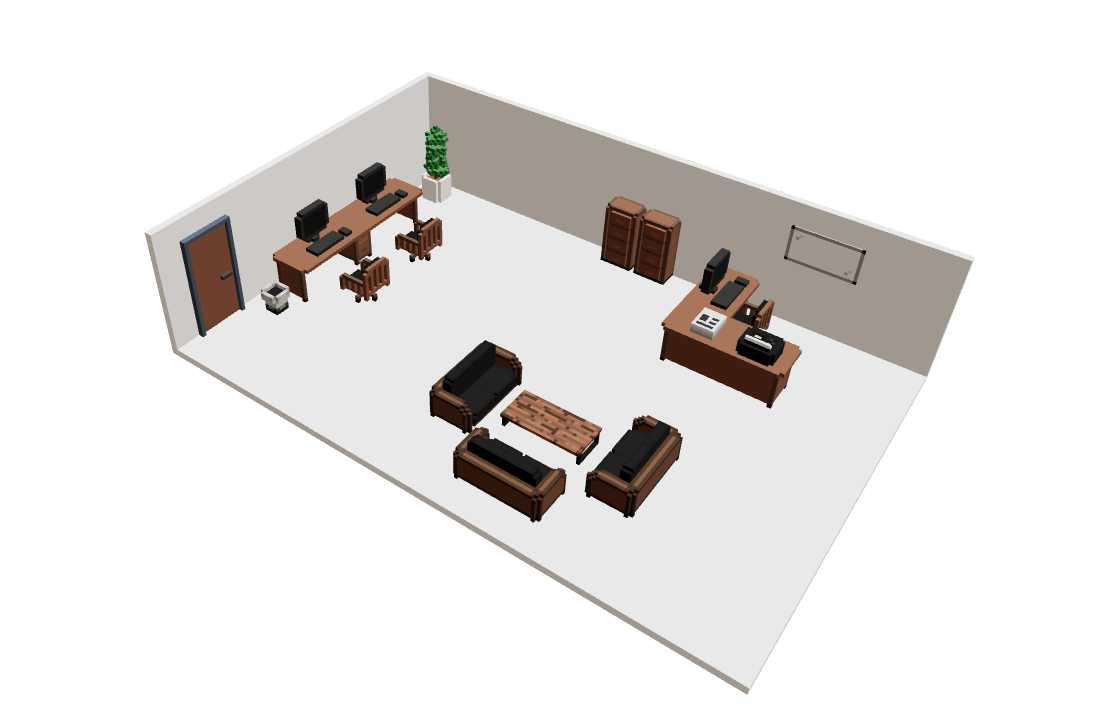
\includegraphics[width=5cm, height=4cm]{office.png}
          \end{center}
    \item Home - Dave's home where he spends time learning and creating.
          \begin{center}
              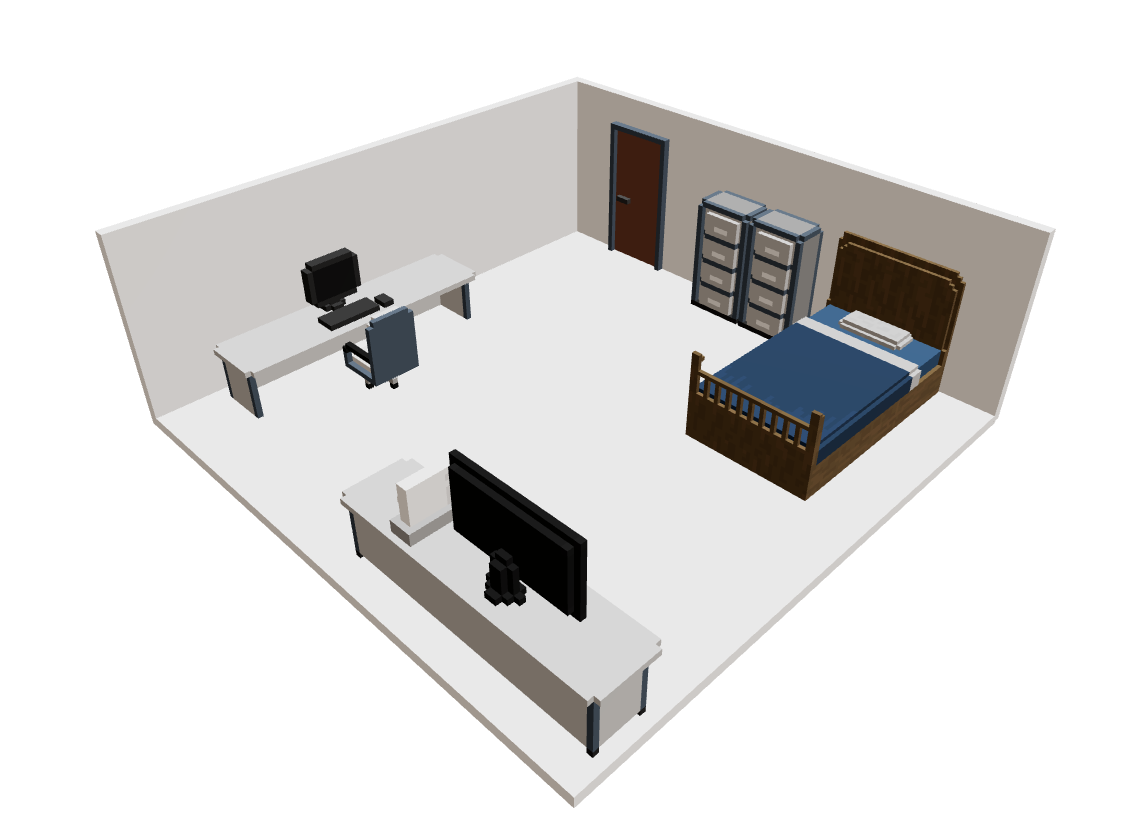
\includegraphics[width=5cm, height=4cm]{home.png}
          \end{center}
    \item Electronics shop - Dave buys circuit parts here from a salesman named Adem Shady
          \begin{center}
              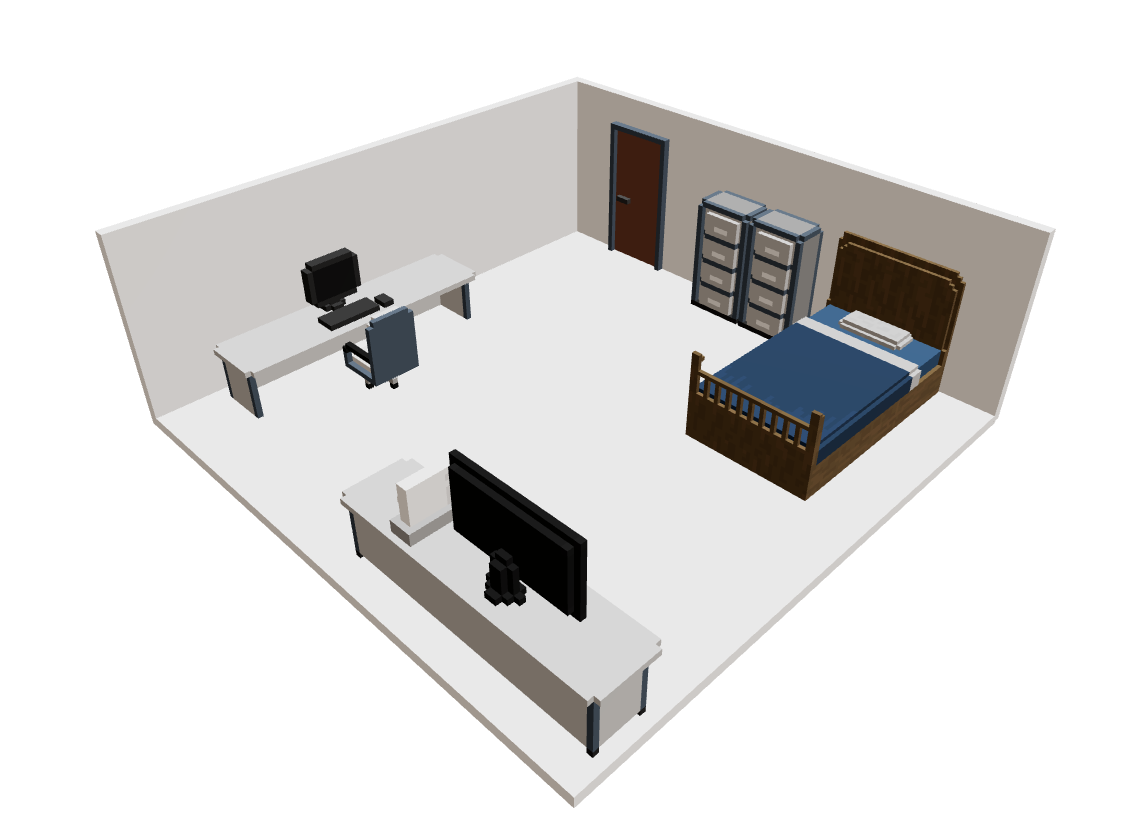
\includegraphics[width=5cm, height=4cm]{home.png}
          \end{center}
\end{enumerate}

Each of the mentioned 3D scenes will contain clickable elements that will open additional UI elements where the gameplay will actually happen 
like for example the circuit editor window.

\subsection{Gameplay}
The goal of the game is too build your own computer that can execute instructions of a predefined format (we made the instructions 
predefined so that we can validate the validity of the made computer by executing predefined programs)







\section{Product market}
\section{Product implementation}

\end{document}